\section{Gamification}\label{sec:gamification}
Gamification is "the process of game-thinking and game mechanics to engage users and solve problems" \cite{Zichermann2011}, i.e. to attract users and keep them coming back to a specific task in order to have them solve problems.

Gamification is used in many areas, for example the game FoldIt, developed by University of Washington in 2008, employs people in folding proteins, which is a job that the brute-force approach of computers does poorly compared to man's natural abilities with regards to spatial reasoning and 3D pattern matching. In 2011 a team of users managed to decode an AIDS-causing monkey virus in just 10 days, a task which had been attempted, unsucessfully, by scientists for 15 years.\cite{Huff2011} Today, the game has almost 500.000 users, using their spare time folding proteins for science for free.\cite{FoldIt2013}

The reason FoldIt works is because it employs game mechanics and dynamics that correlate quite well with primary human desires to keep people interested and engaged in the activity.
Figure \ref{fig:bunchball} show the interaction between human desires such as status, competition and rewards.

\begin{figure}
\begin{figure}[hptb]
  \centering
    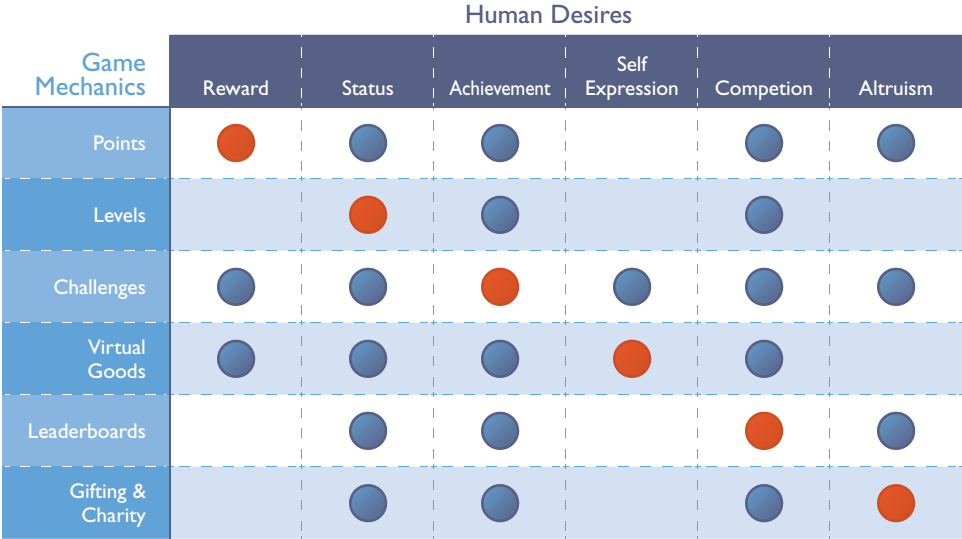
\includegraphics[width=\textwidth]{img/bunchball.png}
  \caption{Interaction between Human desires and Game mechanics}
  \label{fig:bunchball}
\end{figure}
\end{figure}

As can be seen, the human desires can be fulfilled via various game mechanics. In FoldIt, for example, a Leaderboard allows the users to compete against each other either as groups or soloists, which allows both individualists and team players to participate with a feeling of fulfilment. 

If these game mechanics are used, many people will feel entertained in spending time using the product, which is beneficial to a product which, for example, educates the user. In the online application FreeRice the user's desire for altruism is fulfilled via donations of rice grains for completed tasks, while general academic skills are honed, such as vocabulary and basic mathematical proficiency. Again it is possible to join groups, and there is a leaderboard which gives the application an element of competition. \cite{freerice}

